\section{Zielsetzung}
\label{sec:Zielsetzung}
In Versuch 500 wird die Auslösung von Elektronen aus einer Metalloberfläche durch Bestrahlung mit Photonen untersucht.
Dabei wird die Abhängigkeit der Energie der ausgelösten Elektronen von der Wellenlänge des einfallenden Lichts beobachtet.

\section{Theorie}
\label{sec:Theorie}
Licht lässt sich klassisch nicht eindeutig dem Korpuskel- oder dem Wellenmodell zuordnen. So erfordert der lichtelektrische Effekt und der Compton-Effekt eine
Beschreibung als Teilchen. Jedoch lassen sich Phänomene wie die Interferenz oder die Beugung nur mit der Wellentheorie erklären.
Die Quantenmechanik vereint allerdings beide Modelle als Grenzfälle. Lässt sich über eine große Anzahl von Photonen mitteln, so wird die Beschreibung als Welle verwendet.
Bei Wechselwirkungen des Lichts mit Materie dient das Korpuskelmodell als Beschreibung.
\\
\\
Da beim Photoeffekt eine Wechselwirkung stattfindet, wird die Beschreibung des Photons als Teilchen benötigt. Um den Photoeffekt zu realisieren wird eine Metallplatte (Photokathode)
mit monochromatischem Licht bestrahlt. Gegenüber befindet sich eine Auffängerelektrode, die ein positives Potential im Bezug zur Photokathode aufweist.
Die beiden Platten sind über ein Amperemeter verbunden, wodurch der abfließende Strom gemessen wird. Der Strom entsteht dadurch, dass die Elektronen durch die Potentialdifferenz
zur Auffängerelektrode hin beschleunigt werden. Der schematische Aufbau einer solchen Anordnung ist in \autoref{fig:schema} skizziert.
\begin{figure}[H]
    \centering
    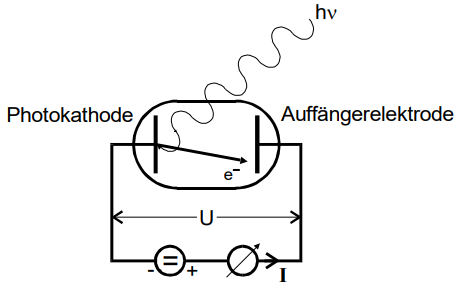
\includegraphics[width=0.5\textwidth]{img/schema.png}
    \caption{Schematischer Aufbau zur Herbeiführung des Photoeffekts \cite{V500}.}
    \label{fig:schema}
\end{figure}

Beim lichtelektrischen Effekt gilt, dass sich die Anzahl der herausgelösten Elektronen proportional zur Lichtintensität verhält und die maximale kinetische Energie der Elektronen
proportional zur Lichtfrequent und unabhängig von der Lichtintensität ist. 
Desweiteren existiert eine Grenzfrequenz unter der der Effekt nicht auftritt.
Klassisch ist dieses Verhalten nicht mit dem Wellenmodell vereinbar. Wird nun jedoch angenommen, dass sich die Energie in einem infinitesimalen Teilchen konzentriert, ist das
genannte Verhalten erklärbar. Diese infinitesimalen Teilchen werden Photonen genannt. Ihre Energie berechnet sich mit
\begin{equation*}
    E_{Ph} = h \cdot f.
\end{equation*}
Dabei ist $E_Ph$ die Photonenenergie, $h$ das Plank'sche Wirkungsquantum und $f$ die Frequenz des Lichtes.
Beim Photoeffekt wird diese Energie beim Auftreffen auf das Kathodenmaterial auf die Elektronen übertragen. Ist die Energie des Photons groß genug, um die 
Austrittsarbeit $A_k$ zu leisten, verlässt das Elektron die Platte. Die Austrittsarbeit $A_k$ ist dabei materialspezifisch. Die überschüssige $E_{Ph}$ erhält dann das 
herausgelöste Elektron als kinetische Energie $E_{kin}$. Folglich gilt
\begin{equation}\label{eq:energie_e}
    hf = E_{kin} + A_k.
\end{equation}
Daraus lässt sich auch direkt ein Schluss auf die Grenzfrequenz ziehen. Gilt nämlich
\begin{equation*}
    f < \frac{A_k}{h}
\end{equation*}
so kann der Photoeffekt nicht mehr auftreten.

\subsection{Konkrete Realisierung des Photoeffekts}
In der genutzten Apperatur zur Untersuchung des Photoeffekts wird ein vakuumierter Glaskolben als Photozelle genutzt. Der Aufbau ist in \autoref{fig:photozelle} skizziert.
Wie aus der Abbildung hervorgeht wird auf der Innenseite des Kolbens eine Metallschicht aufgedampft, die dann als Photokathode dient. Ein um die Photokathode laufender Draht
ist die Anode.

\begin{figure}[H]
    \centering
    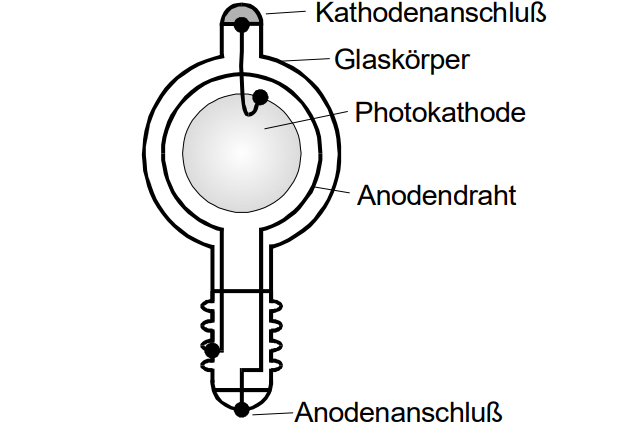
\includegraphics[width=0.5\textwidth]{img/photozelle.png}
    \caption{Aufbau der genutzten Photozelle \cite{V500}.}
    \label{fig:photozelle}
\end{figure}

An die Photozelle wird über den Kathodenanschluss ein externes elektrisches Feld angelegt. Weiterhin werden also die Elektronen durch monochromatisches Licht aus der Oberfläche gelöst, jedoch werden sie jetzt, je nach Orientierung des Feldes,
beschleunigt oder abgebremst. 
Ist ein Gegenfeld angelegt, so lässt sich ein Rückschluss auf die Energie der Elektronen ziehen, denn nun können nur noch Elektronen zur Anode gelangen, deren Energie größer
als $e_0 U$ ist. Zusätzlich wird der Strom gemessen, der von der Kathode zur Anode fließt.
Dieser Strom hört spätestens auf zu fließen wenn 
\begin{equation}\label{eq:ekin}
    e_0 U_g = \frac{m_0 v_{max}^2}{2} 
\end{equation}
gilt. Dabei ist $e_0$ die Elementarladung, $U_g$ die Gegenspannung, $m_0$ die Ruhemasse des Elektrons und $v_{max}$ die Geschwindigkeit der schnellsten Elektronen.
Aus der Gegenspannung ist nun die kinetische Energie der Elektronen bestimmbar. Mit \autoref{eq:energie_e} und \autoref{eq:ekin} gilt nun also
\begin{equation}\label{eq:Elektron_max}
    E_{Ph} = hf = E_{kin} + A_k = e_0 U + A_k.
\end{equation}
Dieser Weg der Bestimmung der Elektronenenergie wird Gegenfeldmethode genannt.

\subsection{Bremsspannung und der daraus resultierende Stromverlauf}
\autoref{eq:Elektron_max} tätigt aber nur eine Aussage über die Elektronen maximaler Energie und den daraus resultierenden 
Strom. In der Realität sinkt der Strom bereits, wenn nicht mehr alle Elektronen von der Kathode zur Anode kommen, d.h. der Strom wird nicht schlagartig $I_{Ph} = 0$ sondern
sinkt mit steigender Gegenspannung ab. Die Strom-Spannungskurve hat in etwa die Form wie in \autoref{fig:bremsspannung}. Ebenfalls ist in \autoref{fig:bremsspannung} zu sehen, dass, wie bereits erläutert, der Strom bei $U = U_g$ nicht mehr messbar ist.

\begin{figure}[H]
    \centering
    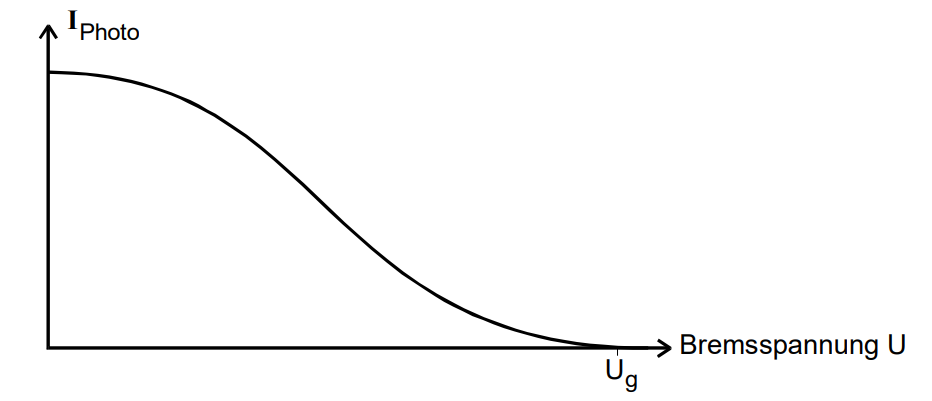
\includegraphics[width=0.8\textwidth]{img/bremsspannung.png}
    \caption{Photostrom $I_{Ph}$ in Abhängigkeit der Bremsspannung $U$ \cite{V500}.}
    \label{fig:bremsspannung}
\end{figure}

\subsection{Aussagen über die Elektronenenergie und auftretende Probleme}
Die Fermi-Dirac-Statistik tätigt eine Aussage über die Energieverteilung in Festkörpern. Da hier jedoch nicht gewährleistet werden kann, dass alle Elektronen die
flächenmäßig kleine Anode erreichen, ist die Fermi-Dirac-Statistik nur bedingt gültig. Nützlich ist aber, dass sich die Spannung quadratisch zum Photostrom verhält:
\begin{equation*}
    I_{Ph} \sim U^2.
\end{equation*}
Es gibt noch einen weiteren Grund, aus dem die Elektronen die Anode nicht erreichen könnten. Denn wenn Anode und Kathode über ein Messgerät elektrisch verbunden sind, 
gleichen sich die Fermi-Niveaus der beiden Materialen auf die gleiche Höhe an. Dies hat zur Folge, dass wenn das Anondenmaterial eine hohe Austrittsarbeit $A_A$
besitzt, sodass $hf < A_A$ gilt, auch kein Photostrom auftreten kann selbst wenn $hf > A_k$ ist, da die Elektronen dann nicht energetisch genug sind, um die Potentialdifferenz
zu überwinden. Das Problem lässt sich lösen indem ein beschleunigendes Potential $U_b$ angelegt wird, sodass
\begin{equation*}
    hf + e_0 U_b \geq A_A
\end{equation*}
gilt.